\chapter{The morphological dependance of quenching}\label{morph}

\emph{The work in the following chapter has been published in \citet{smethurst15}.}


By studying the galaxies which  have just left the mass-SFR relation (see top panel of Figure \ref{sfr_mass_col}),  the quenching mechanisms by which this occurs and its morphological dependance can be probed. By investigating the \emph{amount} of quenching that has occurred in the blue cloud, green valley and red sequence; and by comparing that amount across the three populations, constraints can be applied to the many possible quenching theories outlined in Chapter \ref{intro}. 

I have been motivated by a recent result suggesting there are two contrasting evolutionary pathways through the green valley by different morphological types (\citealt{schawinski14}, hereafter S14). Specifically that late-type galaxies quench very slowly and form a nearly static disc population in the green valley, whereas early-type galaxies quench very rapidly, transitioning through the green valley and onto the red sequence in $\sim 1$~Gyr \citep{Wong12}. That study used a toy model to examine quenching across the green valley but did not use statistics to support their conclusions. Here I use the same toy model but implement \starpy ~in order to statistically study the star formation histories of galaxies across the colour magnitude diagram.


\section{Defining the Green Valley}\label{defGV}

To define which of the $126, 316$ galaxies of the \textsc{gz2-galex} sample are in the green valley, I looked to previous definitions in the literature defining the separation between the red sequence and blue cloud. For example, \citet{Baldry04} used a large sample of $66,846$ local galaxies ($0.004 < z < 0.08$) from the SDSS to trace this bimodality by fitting double Gaussians to the colour magnitude diagram without cuts in morphology. Their relation between the $u-r$ colour, $C'_{ur}$, and r-band magnitude, $M_r$, to define the colour cut between the blue and red galaxy populations is defined in their Equation 11 as:
\begin{equation}\label{eqgv}
C'_{ur}(M_{r}) = 2.06 - 0.244 \tanh \left( \frac{M_r + 20.07}{1.09}\right).
\end{equation}

Due to the necessity for NUV photometry in this study, matching to GALEX removed typical `red and dead' galaxies from the \textsc{gz2-galex} sample. It is therefore not appropriate to define the green valley by a visual fit to the  colour magnitude diagram as in S14. For example, the optical $u-r$ colour histograms shown in Figure \ref{fig:cmgvsplit}, split both a complete SDSS sample and the \textsc{gz2-galex} sample in bins of their absolute r-band magnitude and in each case show the position of the green valley at that $M_r$ as defined by \citet{Baldry04}. For the \textsc{gz2-galex} sample at brighter r-band magnitudes (i.e. larger mass), this definition of the green valley seems to intersect with the observed peak at red colours. However, for the larger SDSS sample (from the MPA-JHU catalog; \citealt{kauffmann03, brinchmann04}) this green valley definition does not intersect with the peak at red colours, as this sample is complete, containing the high mass typical red sequence galaxies. Using a visual fit to the green valley of the \textsc{gz2-galex} sample colour-magnitude diagram would therefore cause green valley galaxies to be misclassified as red sequence.


\begin{figure}
\centering{
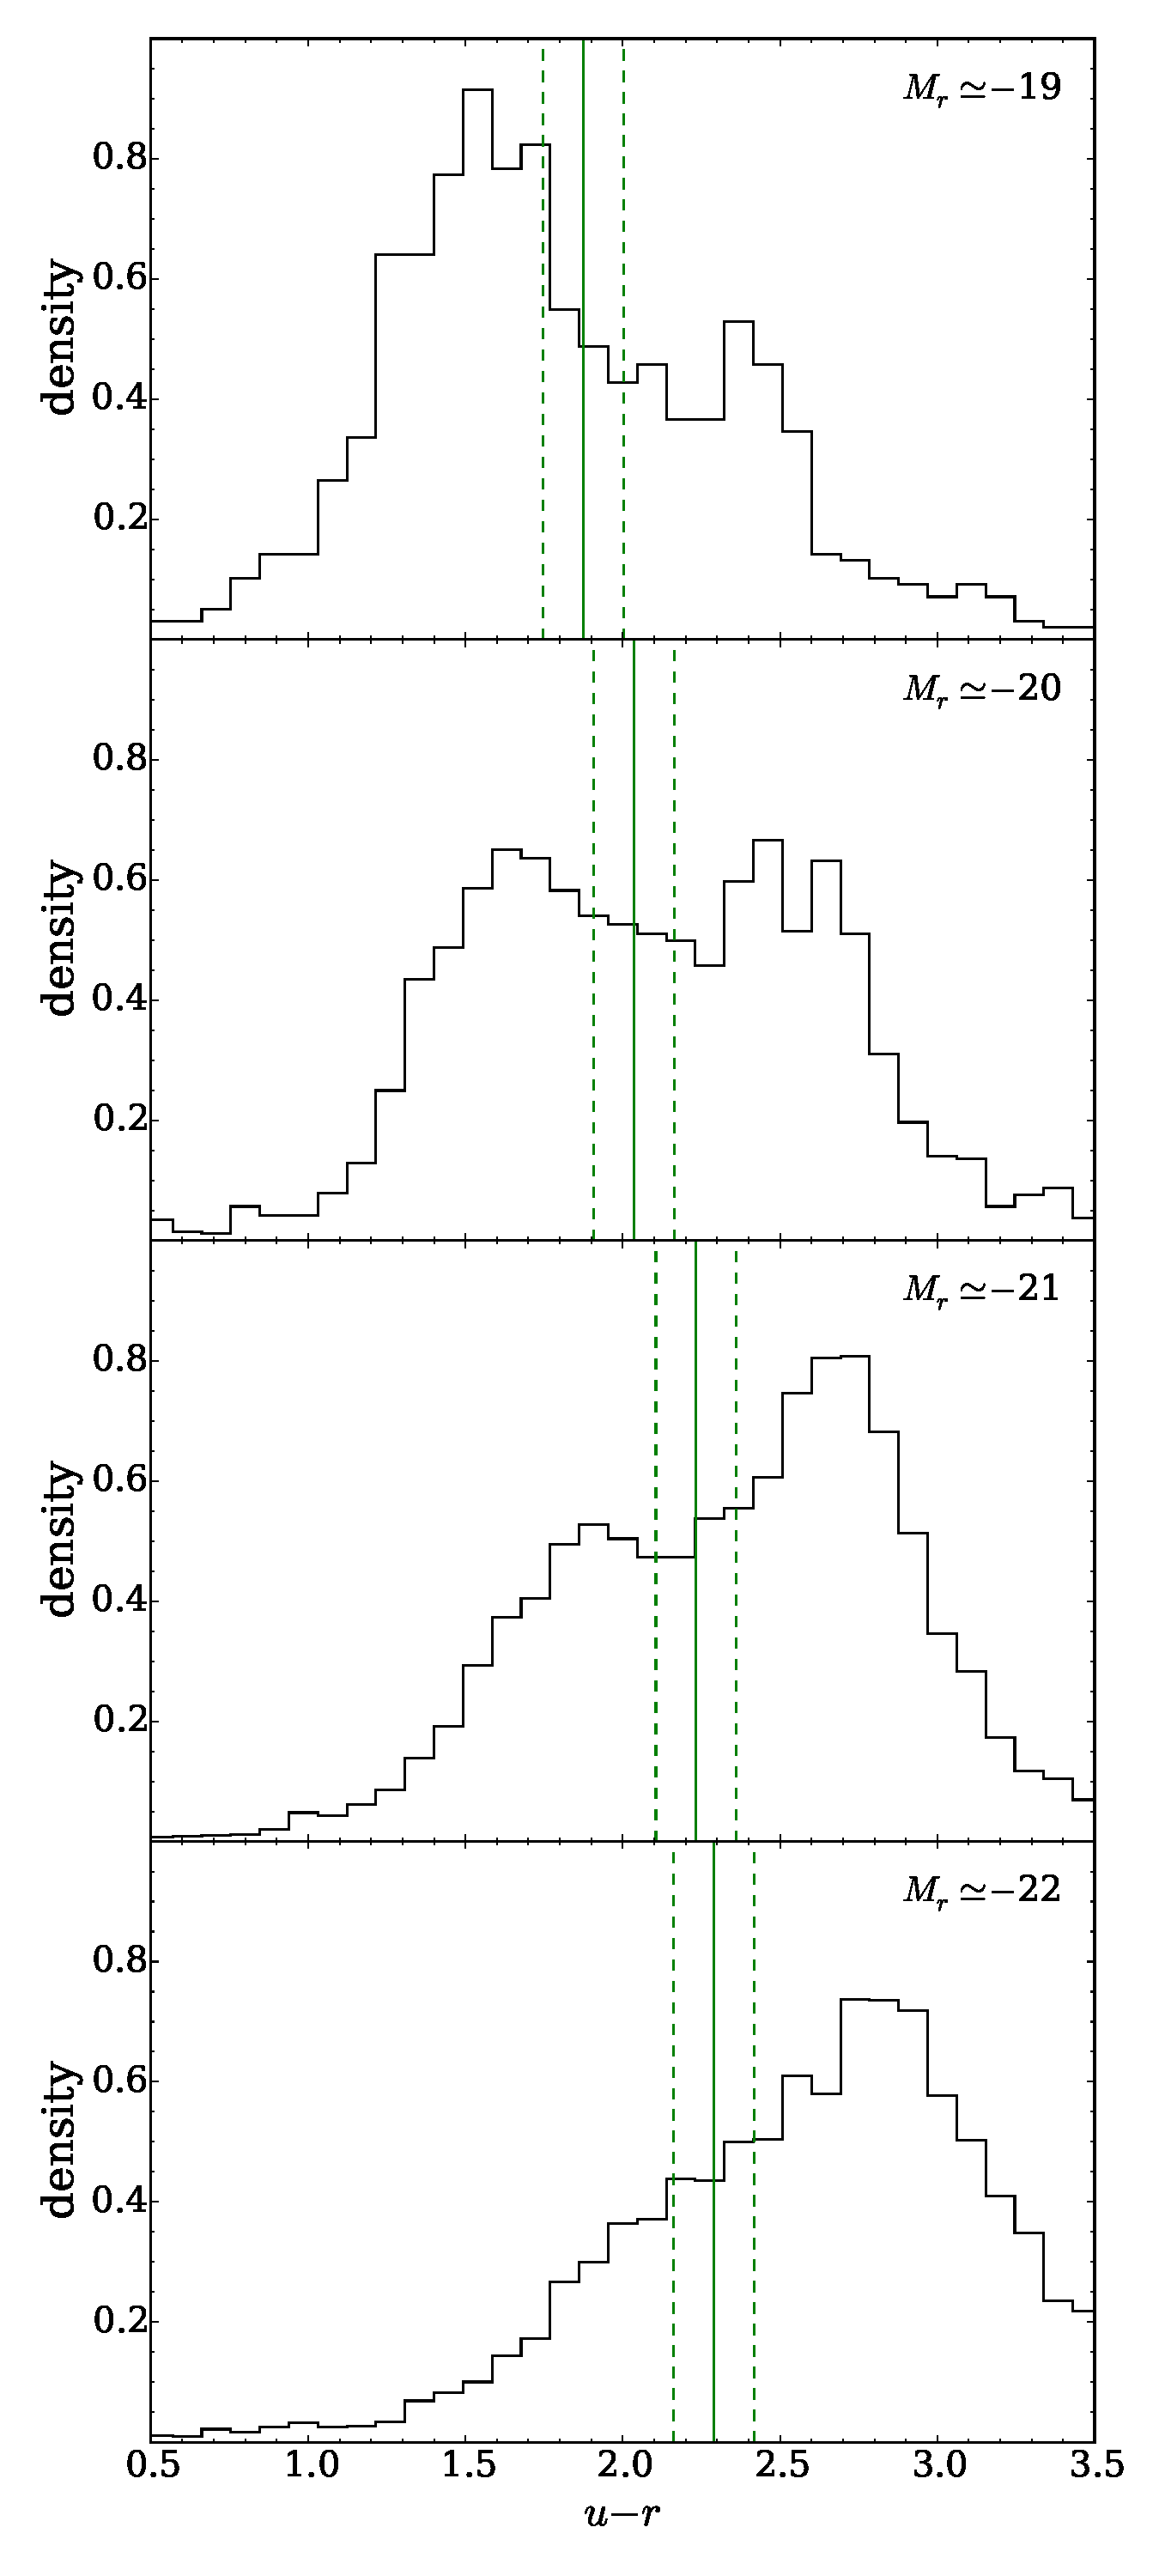
\includegraphics[width=0.49\textwidth]{morphology/sdss_hist_slice.pdf}
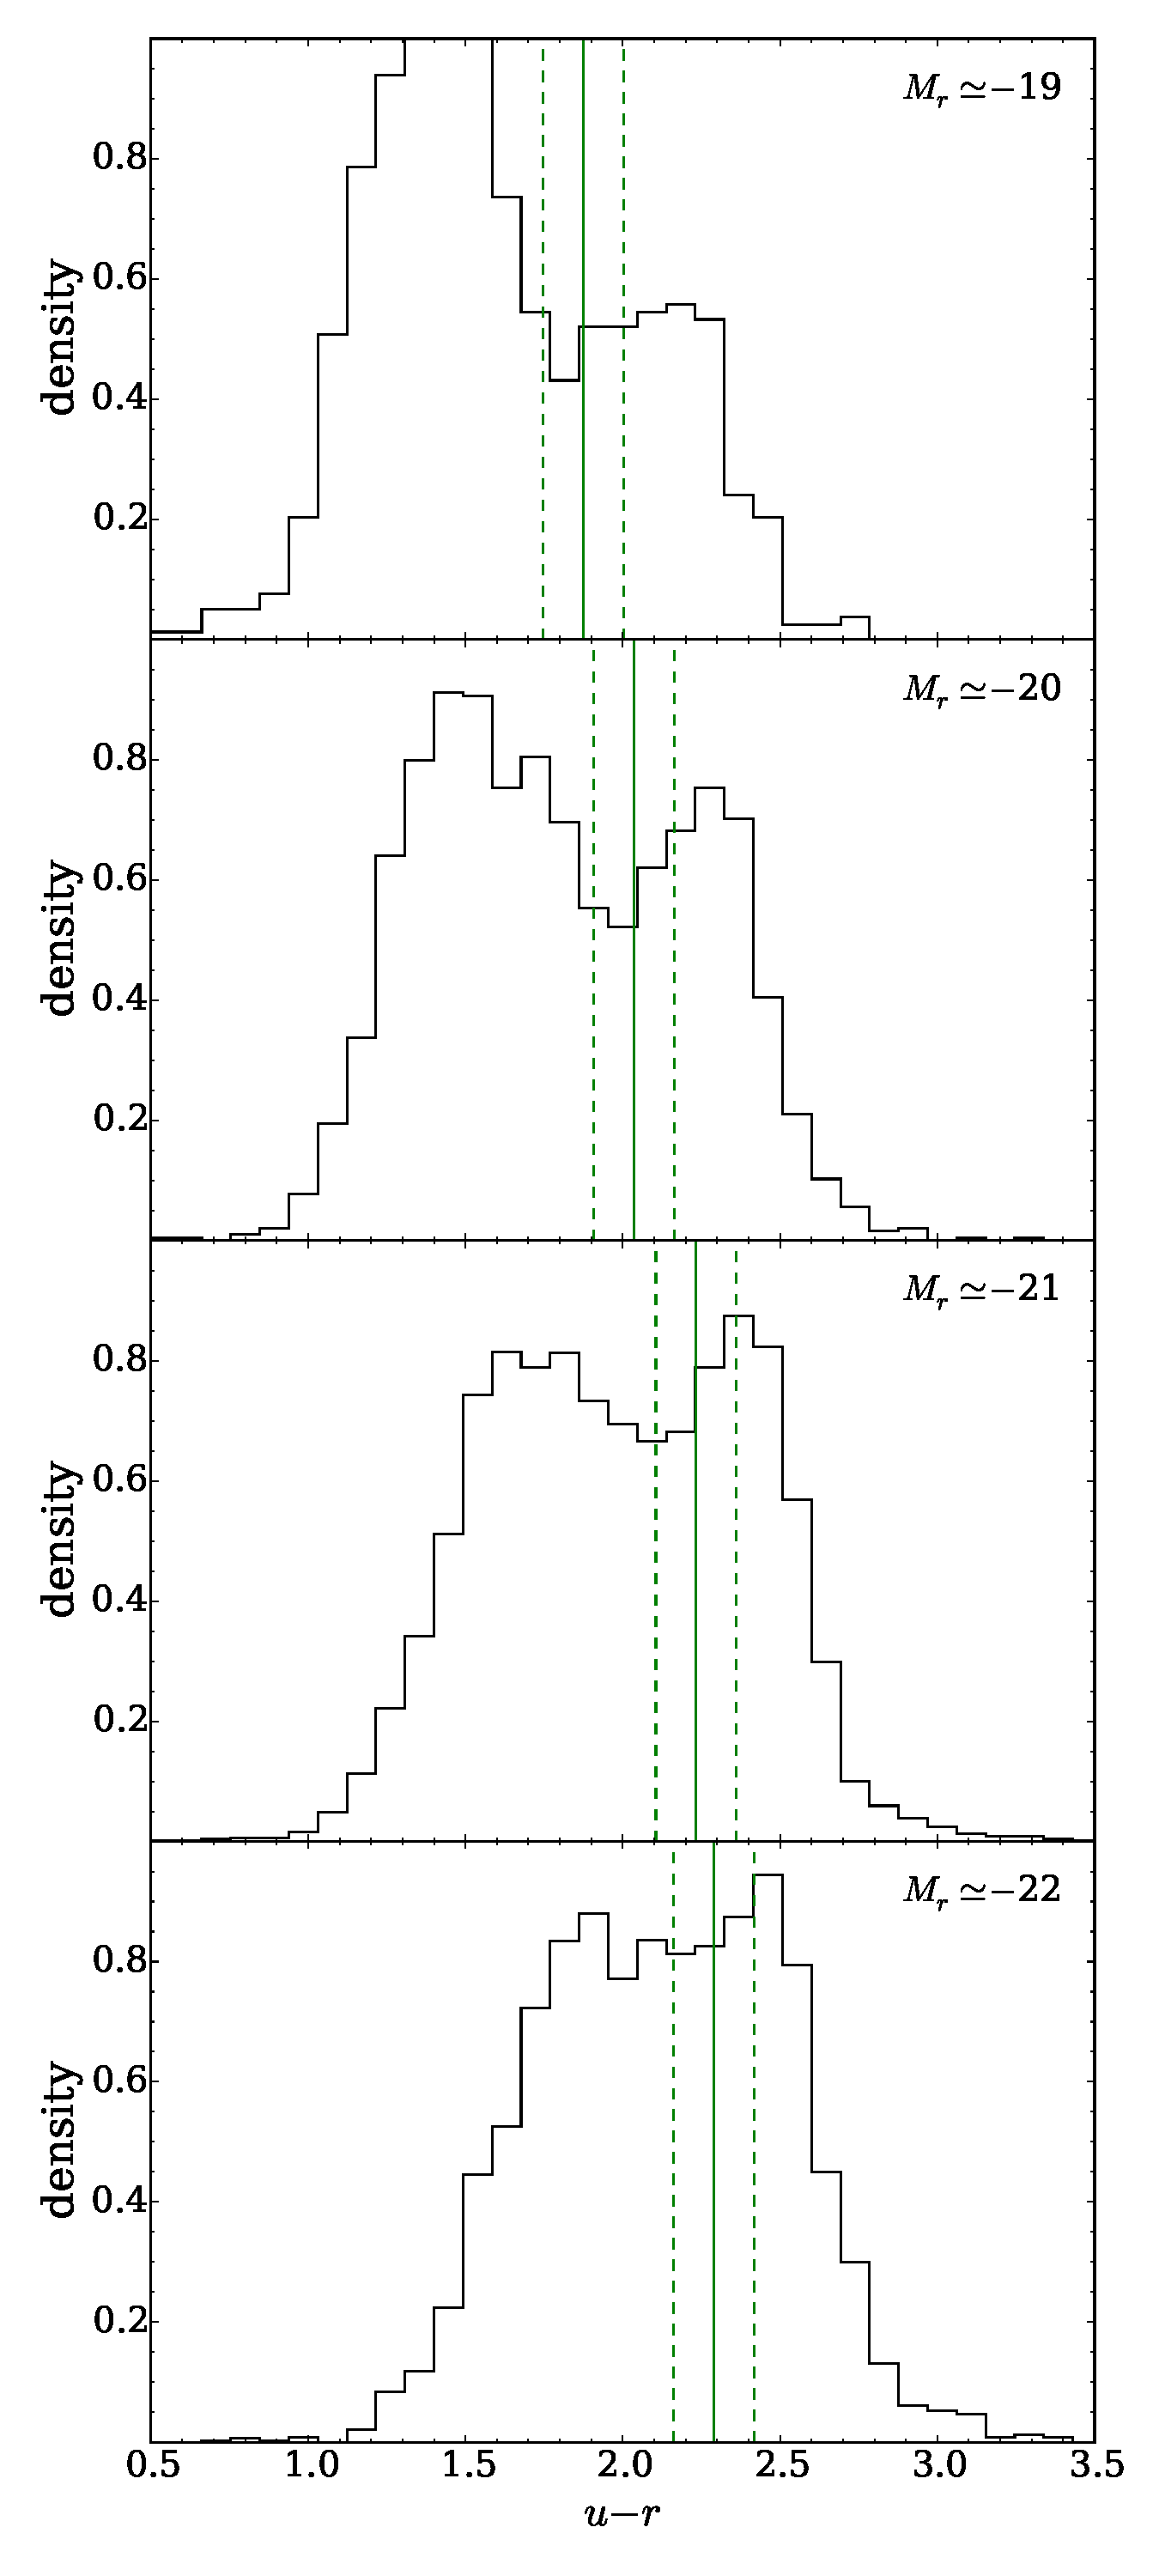
\includegraphics[width=0.49\textwidth]{morphology/galzoo_hist_slice.pdf}}
\caption[Optical $u-r$ colour histograms in absolute r-band magnitude slices of the \textsc{gz2-galex} and Baldry et al. (2004) complete SDSS samples]{Optical $u-r$ colour histograms, sliced in absolute r-band magnitude for a complete SDSS sample (MPA-JHU catalog; left) and for the \textsc{gz2-galex} sample (right). In each panel the definition between the blue cloud and the red sequence from \citet{Baldry04} is shown by the dashed line (as defined in Equation~\ref{eqgv}); the solid lines show $\pm 1\sigma$ either side of this definition.}
\label{fig:cmgvsplit}
\end{figure}

I therefore adopt the \citet{Baldry04} green valley definition for this study which is shown in Figure~\ref{fig:CMGV} by the dashed line in comparison to both the \textsc{gz2-galex} sample (left) and the SDSS data used for the fit by \cite[][right]{Baldry04}. Any galaxy within $\pm 1\sigma$ of this relationship, shown by the solid lines in Figure~\ref{fig:CMGV}, is therefore considered a green valley galaxy. Only $47\%$ of the red sequence galaxies present in the entire Galaxy Zoo 2 sample are present in the \textsc{gz2-galex} sample, as opposed to $72\%$ of the blue cloud and $53\%$ of the green valley galaxies. 

However, although the galaxies identified as residing on the red sequence within the \textsc{gz2-galex} sample have NUV detections, this does not mean they are not representative of a typical red sequence `red and dead' galaxy. \cite{ko13} show that in a sample of quiescent red-sequence galaxies without $\mathrm{H}\alpha$ emission (i.e. without spectral indication of recent star formation), $26\%$ show NUV excess emission and that the fraction with recent star formation is $39\%$. Of the $48\%$ of \textsc{gz2-galex} galaxies classified as below the main sequence using the definition from \citet[][see Section~\ref{qmod}]{peng10}, $44\%$ of these galaxies lie on the red sequence ($94\%$ of all the red sequence galaxies; see Table ~\ref{table:qsubs}). I am therefore confident that the galaxies within the \textsc{gz2-galex} sample will be representative of galaxies across the colour magnitude diagram.

\begin{figure*}
\centering{
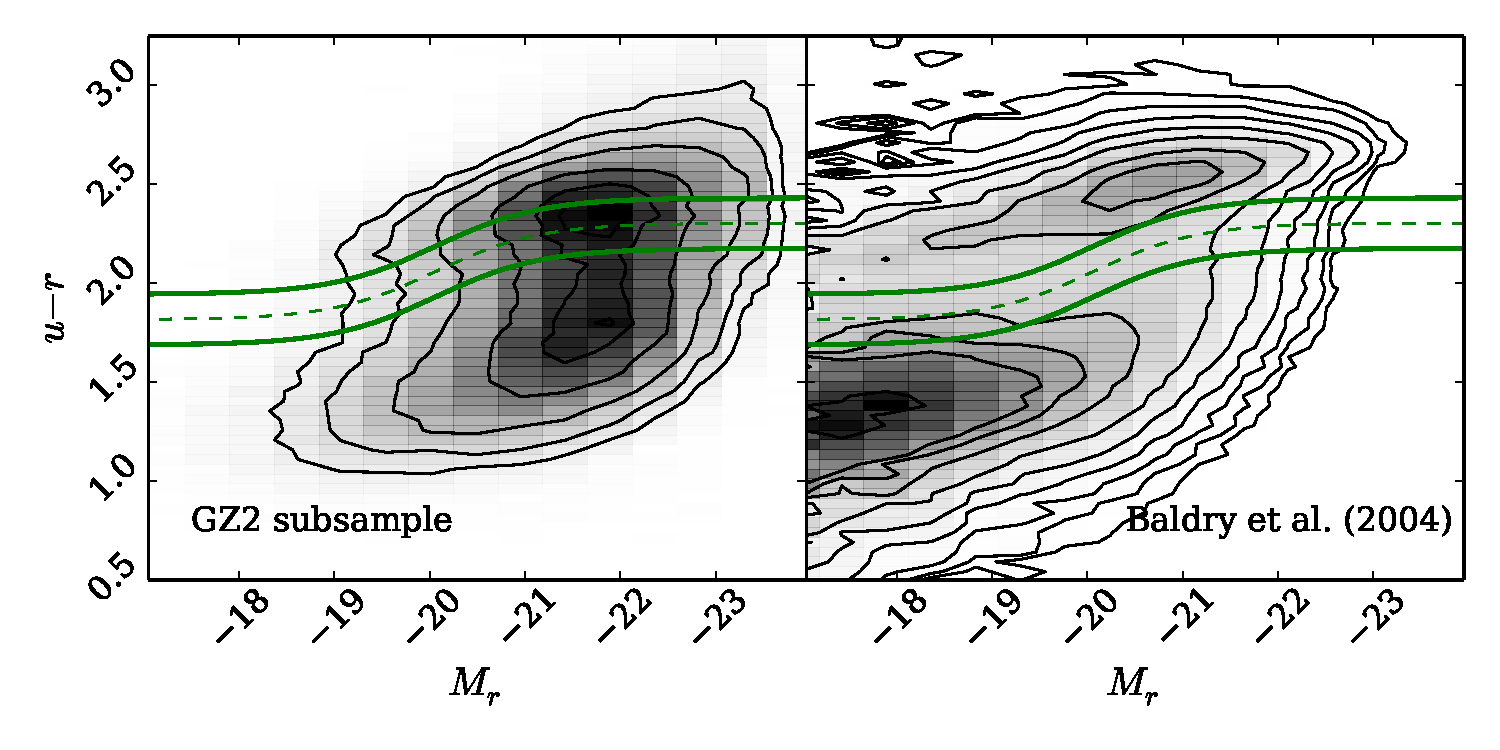
\includegraphics[width=\textwidth]{morphology/col_mag_GV_Baldry_data.pdf}}
\caption[Colour-magnitude diagram showing the location of the Baldry et al. (2004) green valley definition]{Colour-magnitude diagram for the \textsc{gz2-galex} sample (left) and the SDSS sample from \citet[][right]{Baldry04}. In both panels the definition between the blue cloud and the red sequence from \citet{Baldry04} is shown by the dashed line, as defined in Equation~\ref{eqgv}. The solid lines show $\pm 1\sigma$ either side of this definition; any galaxy within the boundary of these two solid lines is considered a green valley galaxy. The lack of red sequence galaxies due to the necessity for NUV GALEX colours skews the apparent location of the green valley in the \textsc{gz2-galex} sample, therefore a literature definition of the green valley is used to ensure galaxies are correctly classified.}
\label{fig:CMGV}
\end{figure*}

The decomposition of the \textsc{gz2-galex} sample into red sequence, green valley and blue cloud galaxies is shown in Tables~\ref{table:subs} and \ref{table:qsubs} along with further subsections by galaxy type and SFR (where available for the \textsc{gz2-galex} sample from the MPA-JHU catalog) respectively. The tables also list the definitions I adopt henceforth for early-type ($p_s~ \geq~0.8$), late-type ($p_d~ \geq~0.8$), smooth-like ($p_s~ >~0.5$), disc-like ($p_d~ >~0.5$), quenched ($\rm{SFR}$ $ < P - 5\sigma$), quenching ($P - 5\sigma < \rm{SFR}$ $< P - \sigma$) and star forming  ($\rm{SFR}$ $> P -\sigma$) galaxies, where $P$ is the SFR as defined by \citet{peng10} for a given stellar mass and observed time (see Equation \ref{eq:peng}). 

\begin{table}
\caption{Table showing the decomposition of the \textsc{gz2-galex} sample by galaxy type into the subsets of the colour-magnitude diagram.}
\begin{tabular*}{\textwidth}{l @{\extracolsep{\fill}}cccc}
\hline
\begin{tabular}[c]{@{}c@{}} {\color{white} -} \\ {\color{white} -}  \end{tabular} & All                                                      & Red Sequence                                              & Green Valley                                              & Blue Cloud \\  \hline 
Smooth-like ($p_s > 0.5$)        & \begin{tabular}[c]{@{}c@{}}42453\\ (33.6\%)\end{tabular} & \begin{tabular}[c]{@{}c@{}}17424\\ (61.9\%)\end{tabular}  & \begin{tabular}[c]{@{}c@{}}10687\\ (44.6\%)\end{tabular}   & \begin{tabular}[c]{@{}c@{}}14342\\ (19.3\%)\end{tabular}  \\ 
Disc-like ($p_d > 0.5$)          & \begin{tabular}[c]{@{}c@{}}83863\\ (80.7\%)\end{tabular} & \begin{tabular}[c]{@{}c@{}}10722\\ (38.1\%)\end{tabular}   & \begin{tabular}[c]{@{}c@{}}13257\\ (55.4\%)\end{tabular}  & \begin{tabular}[c]{@{}c@{}}59884\\ (47.4\%)\end{tabular}  \\
Early-type ($p_s \geq 0.8$) & \begin{tabular}[c]{@{}c@{}}10517\\ (8.3\%)\end{tabular}  & \begin{tabular}[c]{@{}c@{}}5337\\ (18.9\%)\end{tabular}    & \begin{tabular}[c]{@{}c@{}}2496\\ (10.4\%)\end{tabular}    & \begin{tabular}[c]{@{}c@{}}2684\\ (3.6\%)\end{tabular}    \\
Late-type ($p_s \geq 0.8$)  & \begin{tabular}[c]{@{}c@{}}51470\\ (40.9\%)\end{tabular} & \begin{tabular}[c]{@{}c@{}}4493\\ (15.9\%)\end{tabular}    & \begin{tabular}[c]{@{}c@{}}6817\\ (28.5\%)\end{tabular}    & \begin{tabular}[c]{@{}c@{}}40430\\ (54.4\%)\end{tabular}  \\ \hline
\textbf{Total}                       & \begin{tabular}[c]{@{}c@{}}\textbf{126316} \\ (100.0\%)\end{tabular}                                                & \begin{tabular}[c]{@{}c@{}}28146 \\ (22.3\%)\end{tabular} & \begin{tabular}[c]{@{}c@{}}23944 \\ (18.9\%)\end{tabular} & \begin{tabular}[c]{@{}c@{}}74226 \\ (58.7\%)\end{tabular} \\\hline
\end{tabular*}
\label{table:subs}
\end{table}


\begin{table}
\caption{Table showing the decomposition of the \textsc{gz2-galex} sample by their star formation rate in the subsets of the colour-magnitude diagram.}
\begin{tabular*}{\textwidth}{l @{\extracolsep{\fill}}cccc}
\hline
\begin{tabular}[c]{@{}c@{}} {\color{white} -} \\ {\color{white} -}  \end{tabular} 		& All                                                      						& Red Sequence                                              			& Green Valley                                             			 & Blue Cloud \\  \hline 
\begin{tabular}[l]{@{}l@{}}Quenched\\ ($\rm{SFR} < P - 5\sigma$) \end{tabular}	& \begin{tabular}[c]{@{}c@{}}24278\\ (19.7\%)\end{tabular} 			& \begin{tabular}[c]{@{}c@{}}17018\\ (60.9\%)\end{tabular}    & \begin{tabular}[c]{@{}c@{}}6440\\ (27.5\%)\end{tabular}    & \begin{tabular}[c]{@{}c@{}}820\\ (1.1\%)\end{tabular}  \\ 
\begin{tabular}[l]{@{}l@{}}Quenching\\ ($P - 5\sigma < \rm{SFR} < P - \sigma$) \end{tabular}	 & \begin{tabular}[c]{@{}c@{}}34743\\ (28.2\%)\end{tabular}			 & \begin{tabular}[c]{@{}c@{}}9277\\ (33.1\%)\end{tabular}    & \begin{tabular}[c]{@{}c@{}}12181\\ (51.9\%)\end{tabular}    & \begin{tabular}[c]{@{}c@{}}13285\\ (18.6\%)\end{tabular}  \\ 
\begin{tabular}[l]{@{}l@{}}Star Forming  \\ ($\rm{SFR} > P -\sigma$) \end{tabular} & \begin{tabular}[c]{@{}c@{}}63957\\ (52.0\%)\end{tabular} 			& \begin{tabular}[c]{@{}c@{}}1665 \\ (5.9\%)\end{tabular}    & \begin{tabular}[c]{@{}c@{}}4828\\ (20.6\%)\end{tabular}    & \begin{tabular}[c]{@{}c@{}}57464\\ (80.3\%)\end{tabular}  \\ \hline
\textbf{Total}                       		& \begin{tabular}[c]{@{}c@{}}\textbf{122,978} \\ (100.0\%)\end{tabular} & \begin{tabular}[c]{@{}c@{}}27960 \\ (22.7\%)\end{tabular} & \begin{tabular}[c]{@{}c@{}}23449 \\ (19.1\%)\end{tabular} & \begin{tabular}[c]{@{}c@{}}71569 \\ (58.2\%)\end{tabular} \\\hline
\end{tabular*}
\label{table:qsubs}
\end{table}

Figure~\ref{sfr_mass_sub} displays the information shown in Tables \ref{table:subs} \& \ref{table:qsubs} with the SFR against the stellar mass for the \textsc{gz2-galex} sample (where available from the MPA-JHU catalog) by splitting it into blue cloud, green valley red sequence, late- and early-type populations. This figure confirms that the green valley galaxies in the \textsc{gz2-galex} sample are indeed a population which have either left, or begun to leave, the star forming sequence or have some residual star formation still occurring. Figure~\ref{sfr_mass_sub} also reveals that the early-type galaxies of the \textsc{gz2-galex} sample seem to dominate the low and high mass ends of the star forming sequence (shown by the blue solid lines in each panel).  


\begin{figure*}
\centering{
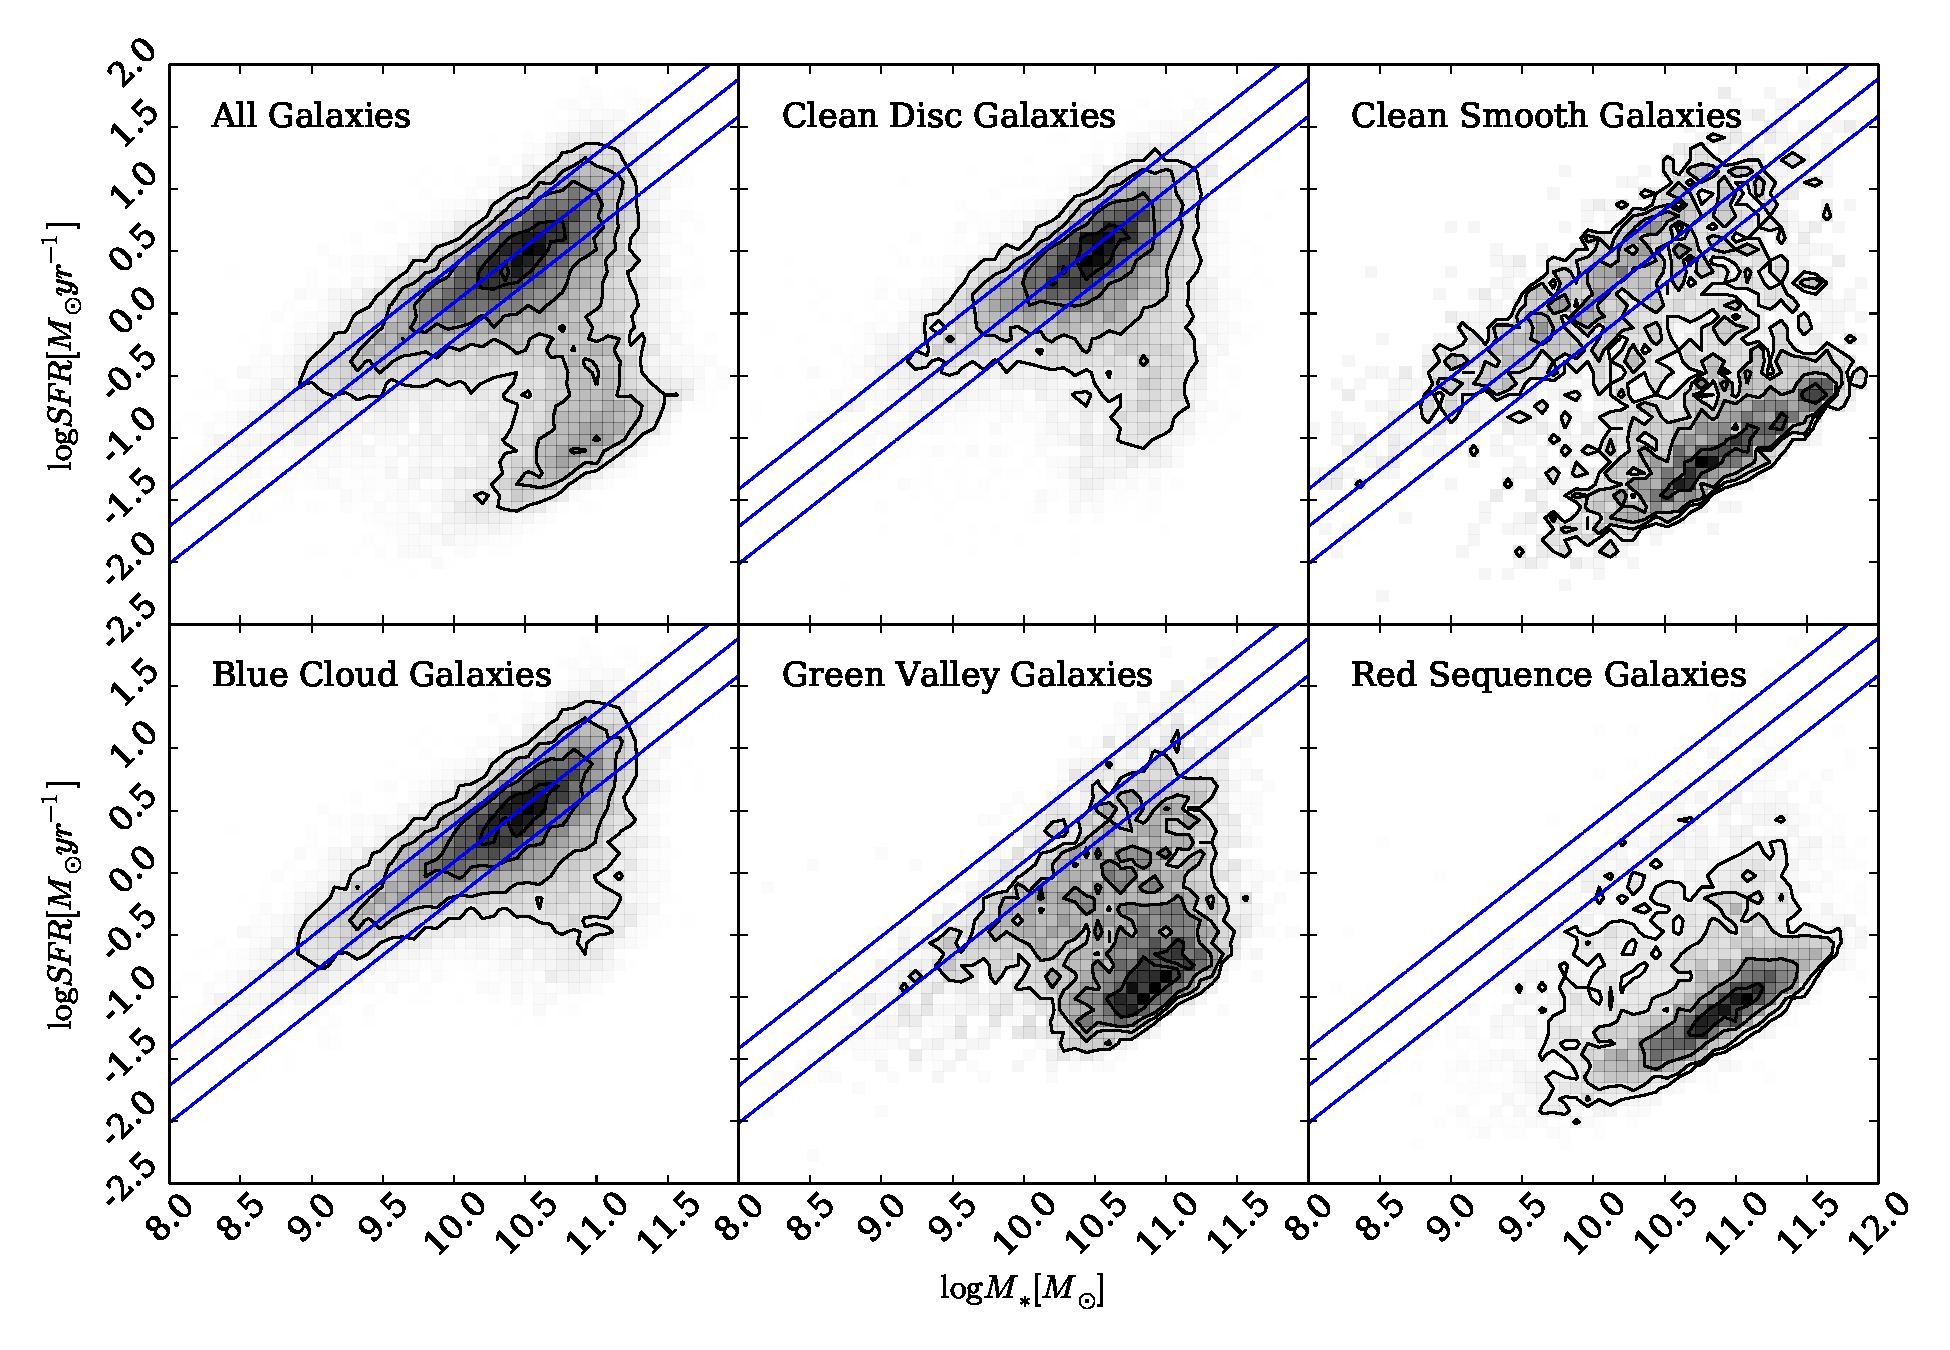
\includegraphics[width=\textwidth]{morphology/sfr_mass_subsets.pdf}}
\caption[SFR-stellar mass plane split by morphology and colour]{Star formation rate against stellar mass for the different populations of galaxies (top row, left to right: all galaxies, late-type galaxies, early-type galaxies; bottom row, left to right: blue cloud, green valley and red sequence galaxies) and how they contribute to the star forming sequence (from \citet{peng10}, shown by the solid blue line with 0.3 dex scatter by the dashed lines). Based on positions in these diagrams, the green valley does appear to be a transitional population between the blue cloud and the red sequence. Detailed analysis of star formation histories can elucidate the nature of the different populations' pathways through the green valley.}
\label{sfr_mass_sub}
\end{figure*}


\section{Results}

The \starpy ~package was run on all galaxies in the \textsc{gz2-galex} sample and the \textsc{popstarpy} method outlined in Section~\ref{popstarpy} was used  to produce Figures~\ref{red_s},~\ref{green_v} \&~\ref{blue_c} for both smooth and disc weighted populations in the red sequence, green valley and blue cloud. The percentages shown in Figures~\ref{red_s},~\ref{green_v} \&~\ref{blue_c} are calculated as the fractions of the population densities located in each region of parameter space for a given population. 

Since the sample contains such a large number of galaxies, these fractions are interpreted as broadly equivalent to the percentage of galaxies in a given population undergoing quenching within the stated timescale range. Although this is not quantitatively exact, it is nevertheless a useful framework for interpreting the population densities.

Also shown in Figure~\ref{fig:bestfit} is the distribution of the median walker positions (the 50th percentile of the posterior probability distribution) of each individual galaxy, split into red, green and blue disc-like ($p_d > 0.5$) and smooth-like ($p_s > 0.5$) populations. These positions were calculated without discarding any walker positions due to low probability and without weighting by the GZ2 morphological vote fractions; therefore this may be more intuitive to understand than Figures~\ref{red_s},~\ref{green_v} \&~\ref{blue_c}.

Although the quenching timescales are continuous in nature, in this Section I refer to rapid, intermediate and slow quenching timescales which correspond to ranges of  $\tau ~\rm{[Gyr]} < 1.0$, $1.0 < \tau ~\rm{[Gyr]} < 2.0$ and $\tau ~\rm{[Gyr]} > 2.0$ respectively for ease of discussion.



\subsection{The Red Sample}\label{rs}

\begin{figure*}
\centering{
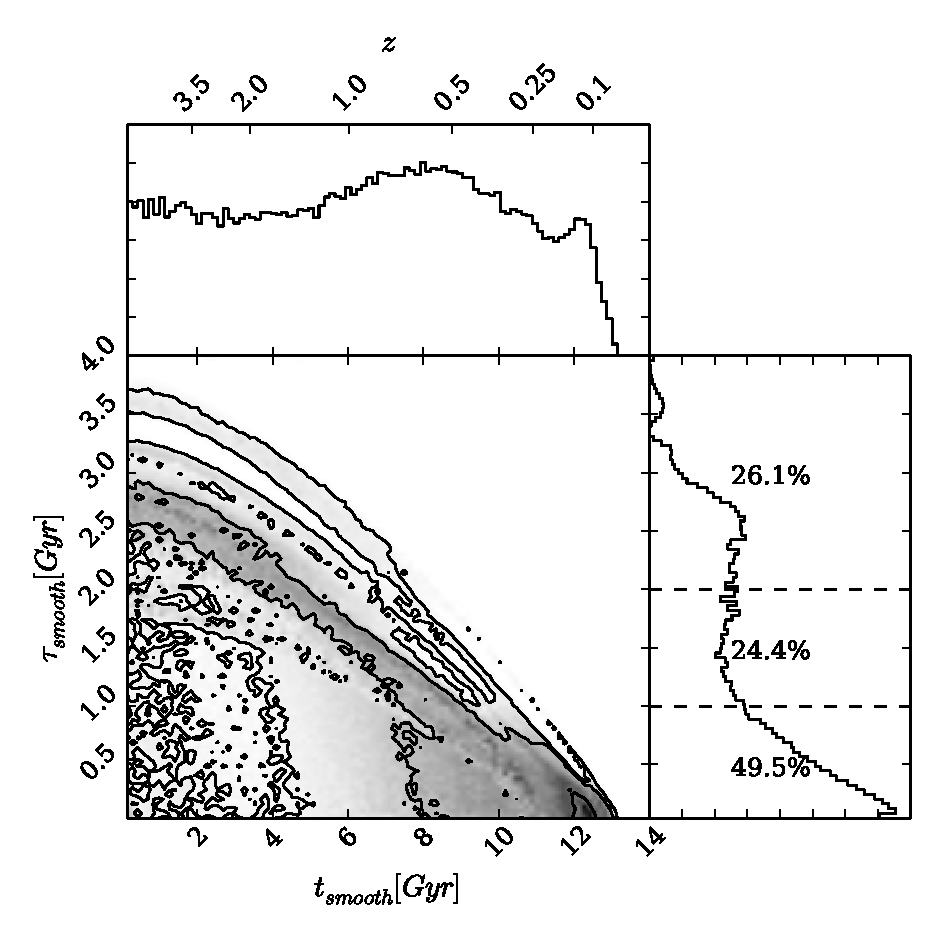
\includegraphics[width=0.55\textwidth]{morphology/red_smooth.pdf}\\
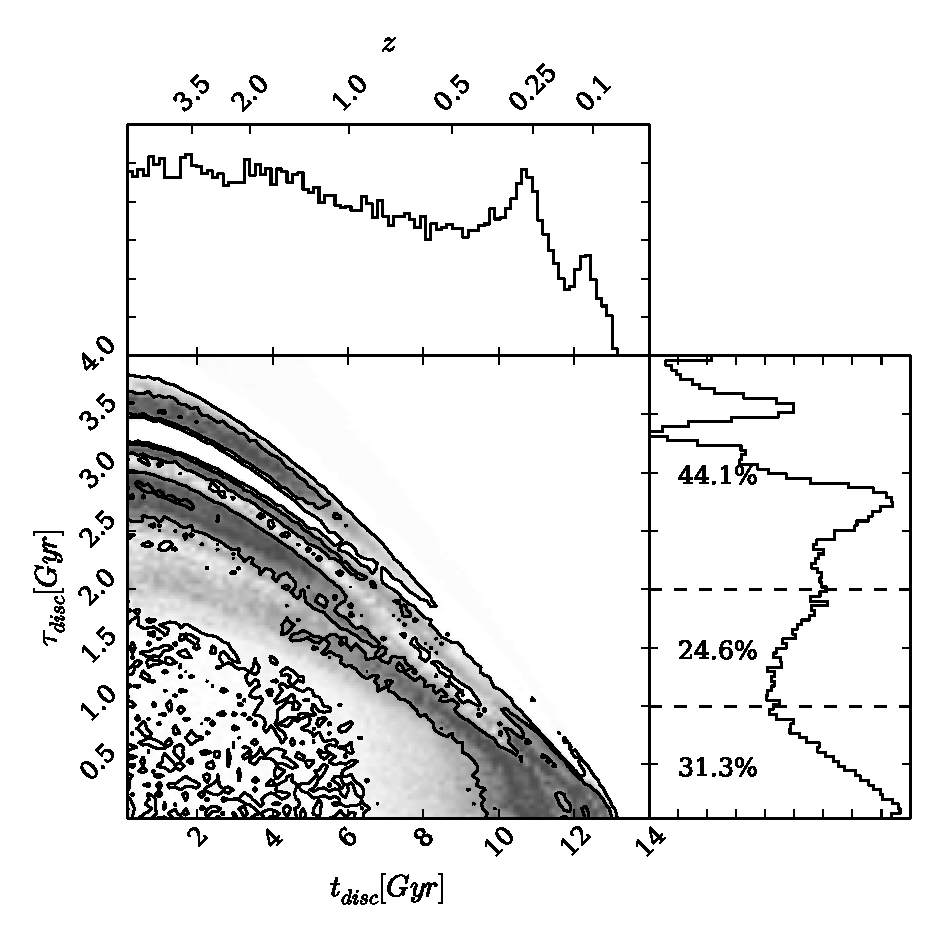
\includegraphics[width=0.55\textwidth]{morphology/red_disc.pdf}}
\caption[Population densities of red smooth and disc galaxies]{Contour plots showing the population densities for red galaxies of the \textsc{gz2-galex} sample, weighted by the morphological vote fractions from GZ2 to give both bulge (top) and disc (bottom) dominated distributions. The histograms show the projection into one dimension for each parameter. The dashed lines show the separation between rapid ($\tau ~\rm{[Gyr]} < 1.0$), intermediate ($1.0 < \tau ~\rm{[Gyr]} < 2.0$) and slow ($\tau ~\rm{[Gyr]} > 2.0$) quenching timescales with the fraction of the combined posterior probability distribution in each region shown (see Section~\ref{stats}).}
\label{red_s}
\end{figure*}

The top panel of Figure~\ref{red_s} reveals that smooth galaxies with red optical colours show a preference $(49.5\%$; see Figure~\ref{red_s}) for rapid quenching timescales across all cosmic time resulting in a very low current SFR. For these smooth red galaxies at early times only, a preference for slow and intermediate timescales in the top panel of Figure~\ref{red_s} is seen. Perhaps this is the influence of intermediate galaxies (with $p_s \sim p_d \sim 0.5$), hence why similar high probability areas exist for both the smooth weighted and disc weighted populations in the top and bottom panels of Figure~\ref{red_s}. This is especially apparent considering there are far more of these intermediate galaxies than those that are definitively early- or late-types (see Table~\ref{table:subs}). These galaxies are those whose morphology cannot be easily distinguished either because they are at a large distance or because they are an S0 galaxy whose morphology can be interpreted by different GZ2 users in different ways. \citet{GZ2} find that S0 galaxies expertly classified by \citet{nair10} are more commonly classified as ellipticals by GZ2 users, but have a significant tail to high disc vote fractions, giving a possible explanation as to the origin of this area of probability.

The bottom panel of Figure~\ref{red_s} reveals that red disc galaxies show similar preferences for rapid $(31.3\%)$ and slow $(44.1\%)$ quenching timescales. The preference for \emph{very} slow ($\tau > 3.0 ~\rm{Gyr}$) quenching timescales (which are not seen in either the green valley or blue cloud, see Figures~\ref{green_v} and~\ref{blue_c}) suggests that these  galaxies have only just reached the red sequence after a very slow evolution across the colour-magnitude diagram. Considering their limited number and the requirement for NUV emission, it is likely that these galaxies are currently on the edge of the red sequence having recently (and finally) moved out of the green valley. Table~\ref{table:subs} shows that $3.9\%$ of the sample are red sequence late-type galaxies, i.e. red late-type spirals. This is, within uncertainties, in agreement with the findings of \citet{masters10c}, who find $\sim6\%$ of late-type spirals are red when defined by a cut in the $g-r$ optical colour (rather than with $u-r$ as used in this investigation) and are at the `blue end of the red sequence'. 

Despite the dominance of slow quenching timescales, the red disc weighted population also show some preference for rapid quenching timescales ($31.3\%$), similar to the red smooth weighted population but with a lower likelihood. Perhaps these rapid quenching timescales can also be attributed to a morphological change, suggesting that the quenching has occurred more rapidly than the morphological change to a bulge dominated system.

Comparing the resultant SFRs for both the smooth and disc weighted populations in Figure~\ref{red_s} by noticing where the areas of high probability lie with respect to the bottom panel of Figure~\ref{pred} (which shows the predicted SFR at an observation time of $t\sim12.8~\rm{Gyr}$, the average `observed' time of the \textsc{gz2-galex} sample) reveals that red disc weighted population with a preference for slow quenching still have some residual star formation occurring, SFR$~\sim0.105 M_{\odot}yr^{-1}$, whereas the smooth galaxies with a dominant preference for rapid quenching have a resultant SFR$~\sim0.0075 M_{\odot}yr^{-1}$. This is approximately 14 times less than the residual SFR still occurring in the red disc weighted population. Within error, this is in agreement with the findings of \citet{tojeiro13} who, by using the VErsatile SPectral Analyses spectral fitting code (VESPA; \citealt{tojeiro07}), found that red late-type spirals show 17 times more recent star formation than red elliptical galaxies.

These results for the red galaxies investigated here with NUV emission, have many implications for green valley galaxies, as all of these systems must have passed through the green valley on their way to the red sequence. 

\subsection{Green Valley Galaxies}\label{gv}

\begin{figure*}
\centering{
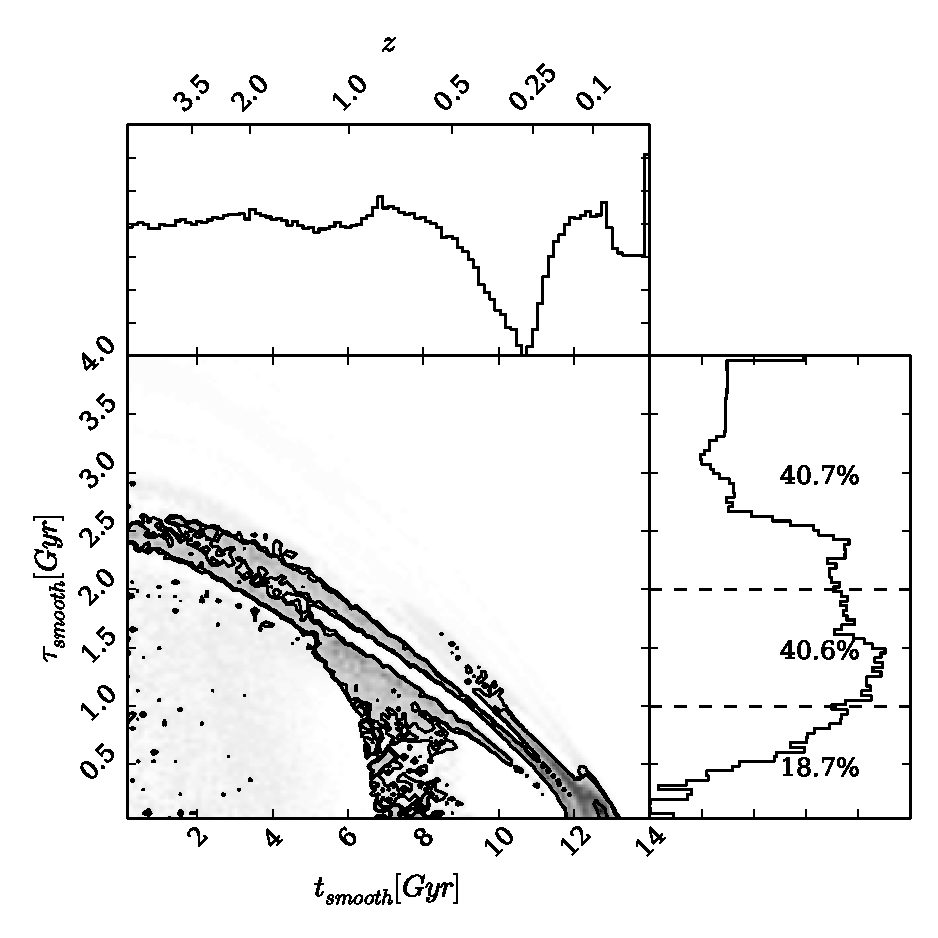
\includegraphics[width=0.55\textwidth]{morphology/green_smooth.pdf}\\
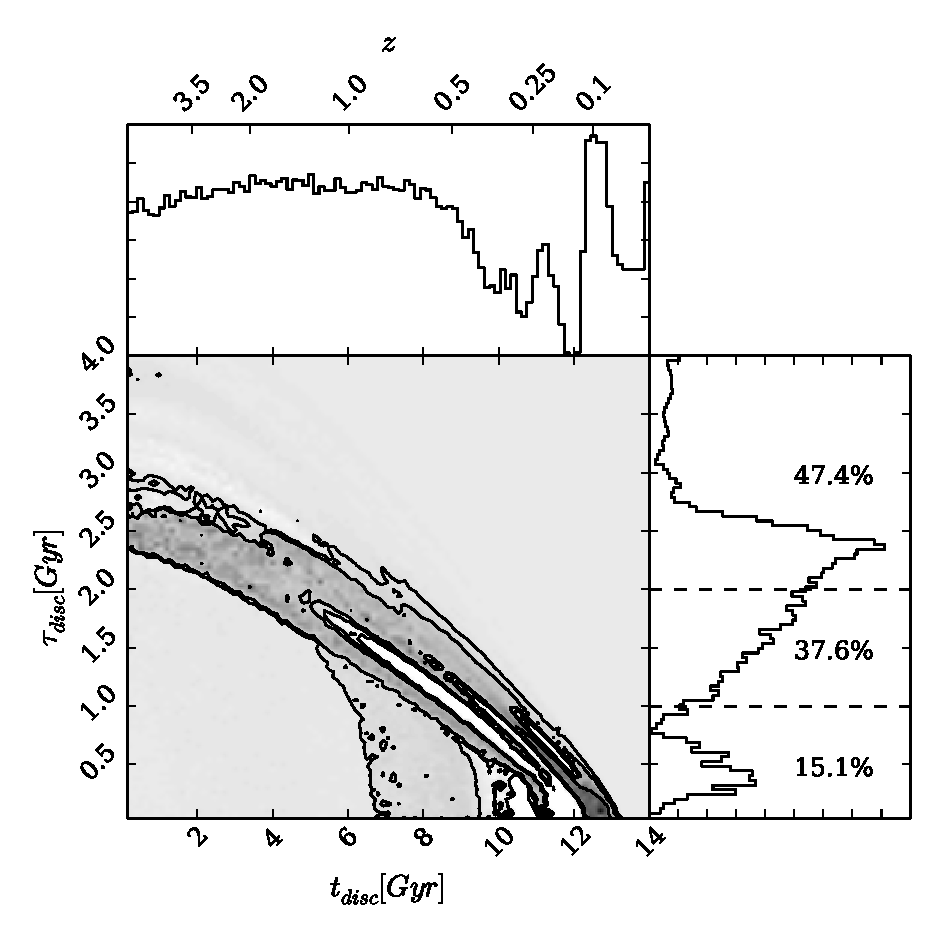
\includegraphics[width=0.55\textwidth]{morphology/green_disc.pdf}}
\caption[Population densities of green smooth and disc galaxies]{Contour plots showing the population densities for green valley galaxies in the \textsc{gz2-galex} sample weighted by the morphological vote fractions from GZ2 to give both bulge (top) and disc (bottom) dominated distributions. The histograms show the projection into one dimension for each parameter. The dashed lines show the separation between rapid ($\tau ~\rm{[Gyr]} < 1.0$), intermediate ($1.0 < \tau ~\rm{[Gyr]} < 2.0$) and slow ($\tau ~\rm{[Gyr]} > 2.0$) quenching timescales with the fraction of the combined posterior probability distribution in each region shown (see Section~\ref{stats}).}
\label{green_v}
\end{figure*}

In Figure~\ref{green_v} similar comparisons for the green valley galaxies can be made to those discussed previously for the red galaxies studied. For the red galaxies, an argument can be made for two possible tracks across the green valley, shown by the bimodal nature of both distributions in $\tau$, with a common area in the intermediate timescale region where the rapid and slow timescales peaked distributions intersect. However in the green valley this intermediate quenching timescale region becomes more significant  (in agreement with the conclusions of \citealt{Gonc12}), particularly for the smooth weighted population (see the top panel of Figure~\ref{green_v}).

The smooth weighted population densities favour these intermediate quenching timescales ($40.6\%$) with some preference for slow quenching at  early times ($z > 1$). The preference for rapid quenching in the smooth population has dropped by over a half compared to the red population, however this will be influenced by the observability of galaxies undergoing such a rapid quench which will spend significantly less time in the transitional population of the green valley. To quantify this, I tested the time spent in the green valley across the $[t, \tau]$ parameter space, which is shown in Figure~\ref{fig:timeingv}. Those galaxies with such a rapid decline in star formation pass so quickly through the green valley and so will be detected at a lower number than those galaxies which have stalled in the green valley with intermediate quenching timescales.  This accounts for the observed number of intermediate galaxies which are present in the green valley and the dominance of rapid timescales detected for the red populations of both morphologies.

\begin{figure*}
\centering{
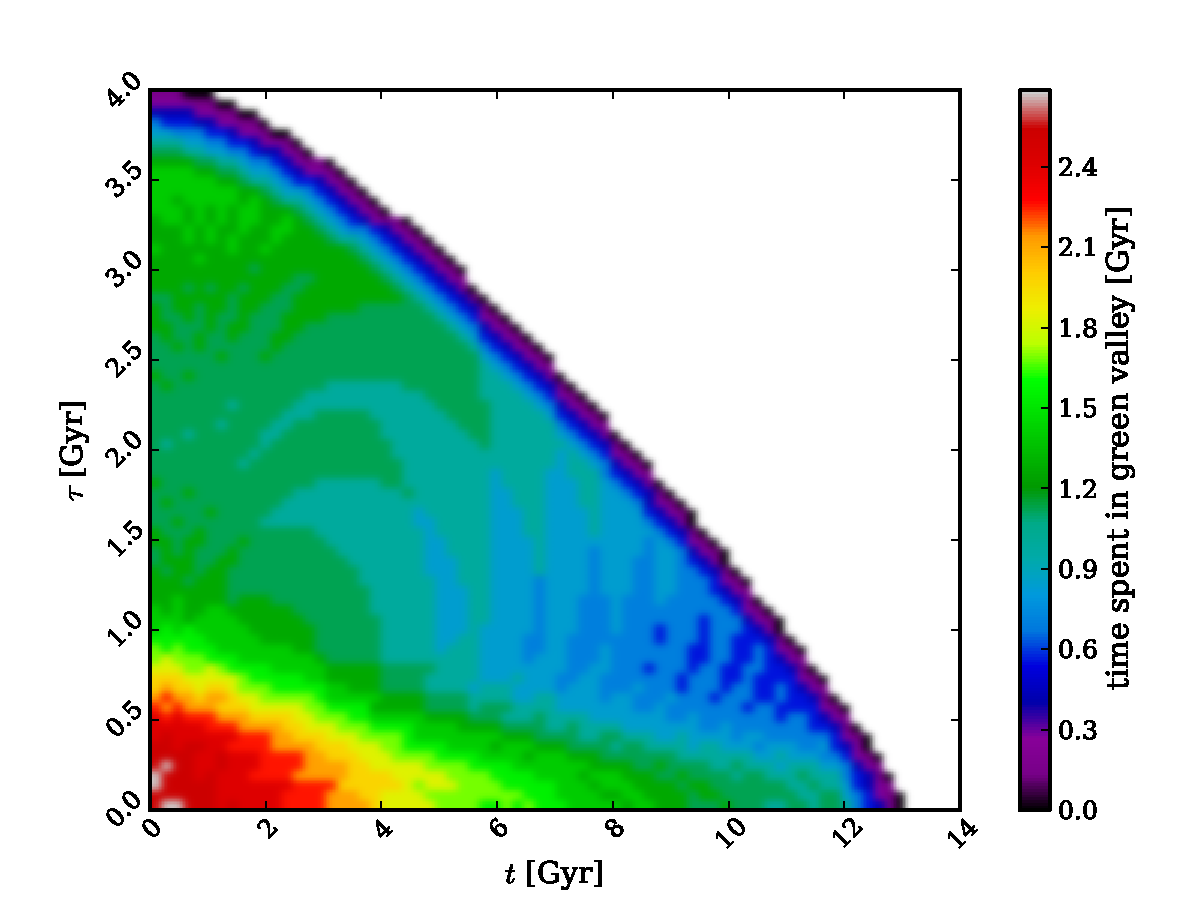
\includegraphics[width=0.9\textwidth]{morphology/green_valley_time.pdf}}
\caption[Time spent in the green valley across parameter space]{Plot showing the time spent in the green valley across the SFH model parameter space by the current epoch. This affects the observability of those galaxies which have quenched rapidly and recently and have passed too quickly through the green valley to be detected. The white region denotes those models with colours that do not enter the green valley by the present cosmic time.}
\label{fig:timeingv}
\end{figure*}

The green valley disc weighted population now overwhelmingly prefer slow quenching timescales ($47.4\%$) with a similar amount of intermediate quenching compared to the smooth weighted parameters ($37.6\%$; see Figure~\ref{green_v}). There is still some preference for galaxies with a star formation history which results in a high current SFR, suggesting there are also some late-type galaxies that have just progressed from the blue cloud into the green valley. 

If Figure~\ref{green_v} to Figure~\ref{red_s} are compared, quenching is seen to occur at later (more recent) cosmic times in the green valley than for red galaxies of both morphological types. Therefore both morphologies are tracing the evolution of the red sequence, confirming that the green valley is indeed a transitional population between blue cloud and red sequence regardless of morphology. Currently as the green valley is observed, its main constituents are very slowly evolving disc-like galaxies along with intermediate- and smooth-like galaxies which pass across it with intermediate timescales within $\sim 1.0-1.5~\rm{Gyr}$.

Given enough time ($t\sim4 - 5~\rm{Gyr}$), the disc galaxies will eventually fully pass through the green valley and make it out to the red sequence (the bottom panel of Figure~\ref{sfr_mass_col} shows galaxies with $\tau > 1.0~\rm{Gyr}$ do not approach the red sequence within $3~\rm{Gyr}$ post quench). This is most likely the origin of the `red spirals'.

Considering that the green valley is a transitional population, the ratio of smooth:disc galaxies that is currently observed in the green valley is expected to evolve into the ratio observed for the red galaxies with NUV emission investigated. Table~\ref{table:subs} shows the ratio of smooth-like : disc-like galaxies in the observed red sequence of the \textsc{gz2-galex} sample is $62:38$ whereas in the green valley it is $45:55$. Making the very simple assumptions that this ratio does not change with redshift and that quenching is the only mechanism which causes a morphological transformation, then $31.2\%$ of the disc-dominated galaxies currently residing in the green valley would have to undergo a morphological change to a bulge-dominated galaxy. The fraction of the density of the green valley disc weighted population occupying the parameter space $\tau < 1.5 ~\rm{Gyr}$ is $29.4\%$, this suggests that quenching mechanisms with these timescales are capable of destroying the disc-dominated structure of galaxies. However this is most likely an overestimate of the timescale that can cause a morphological change because of the observability of those galaxies which undergo such a rapid quench; \citet[][and see Figure~\ref{fig:timeingv}]{Martin07} showed that after considering the time spent in the green valley, the fraction of galaxies undergoing a rapid quench quadruples.


All of this evidence suggests that there are not just two routes for galaxies through the green valley as concluded by S14, but a continuum of quenching timescales which can be divided into three general regimes: rapid ($\tau < 1.0 ~\rm{Gyr}$), intermediate ($1.0 < \tau < 2.0~\rm{Gyr}$) and slow ($\tau > 2.0~\rm{Gyr}$). The intermediate quenching timescales reside in the space between the extremes sampled by the UV/optical diagrams of S14; the inclusion of the intermediate galaxies in this investigation (unlike in S14) and the more precise Bayesian analysis, quantifies this range of $\tau$ and specifically ties the intermediate timescales to all variations of galaxy morphology.

Instead of concluding that \emph{`the green valley is a red herring'} as in S14, one might instead conclude that the \emph{`grass is always redder on the other side'}.


\subsection{Blue Cloud Galaxies}\label{bc}

\begin{figure*}
\centering{
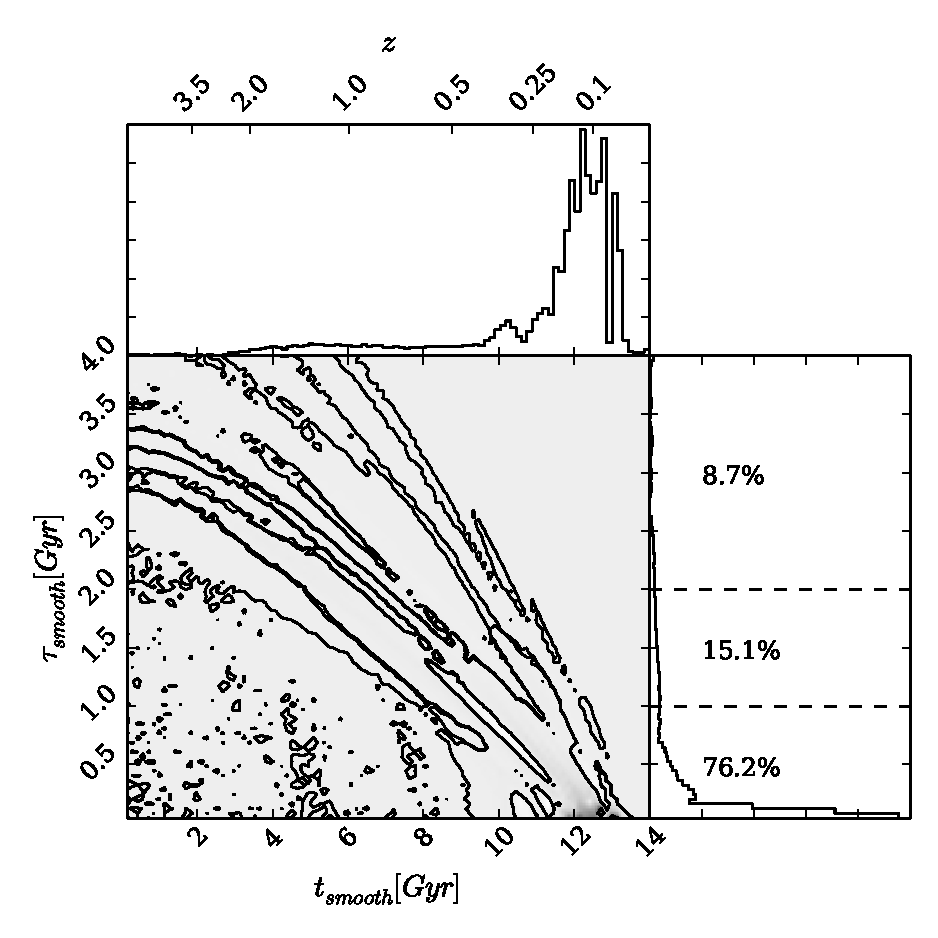
\includegraphics[width=0.55\textwidth]{morphology/blue_smooth.pdf}\\
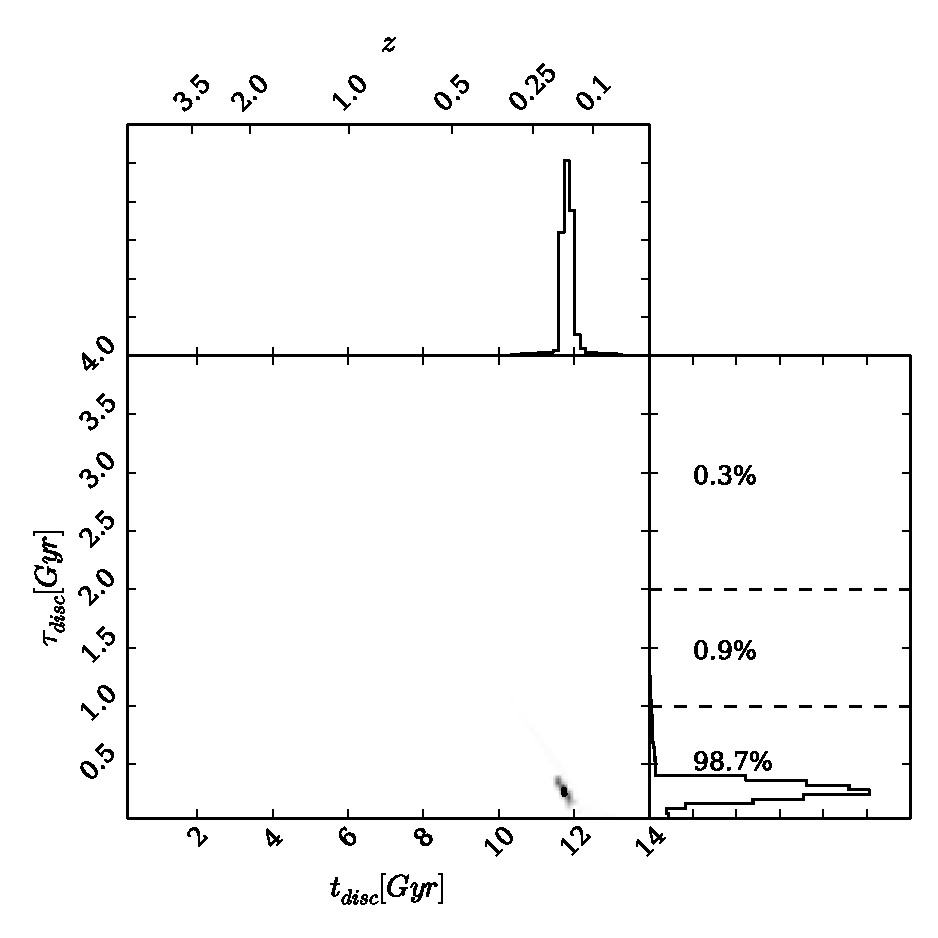
\includegraphics[width=0.55\textwidth]{morphology/blue_disc.pdf}}
\caption[Population densities of blue smooth and disc galaxies]{Contour plots showing the population densities blue cloud galaxies in the \textsc{gz2-galex} sample, weighted by the morphological vote fractions from GZ2 to give both bulge (top) and disc (bottom) dominated distributions. The histograms show the projection into one dimension for each parameter. The dashed lines show the separation between rapid ($\tau ~\rm{[Gyr]} < 1.0$), intermediate ($1.0 < \tau ~\rm{[Gyr]} < 2.0$) and slow ($\tau ~\rm{[Gyr]} > 2.0$) quenching timescales with the fraction of the combined posterior probability distribution in each region shown (see Section~\ref{stats}). Positions with probabilities less than 0.2 are discarded as poorly fit models, therefore unsurprisingly blue cloud galaxies are not well described by a quenching star formation model. }
\label{blue_c}
\end{figure*}

\begin{figure*}
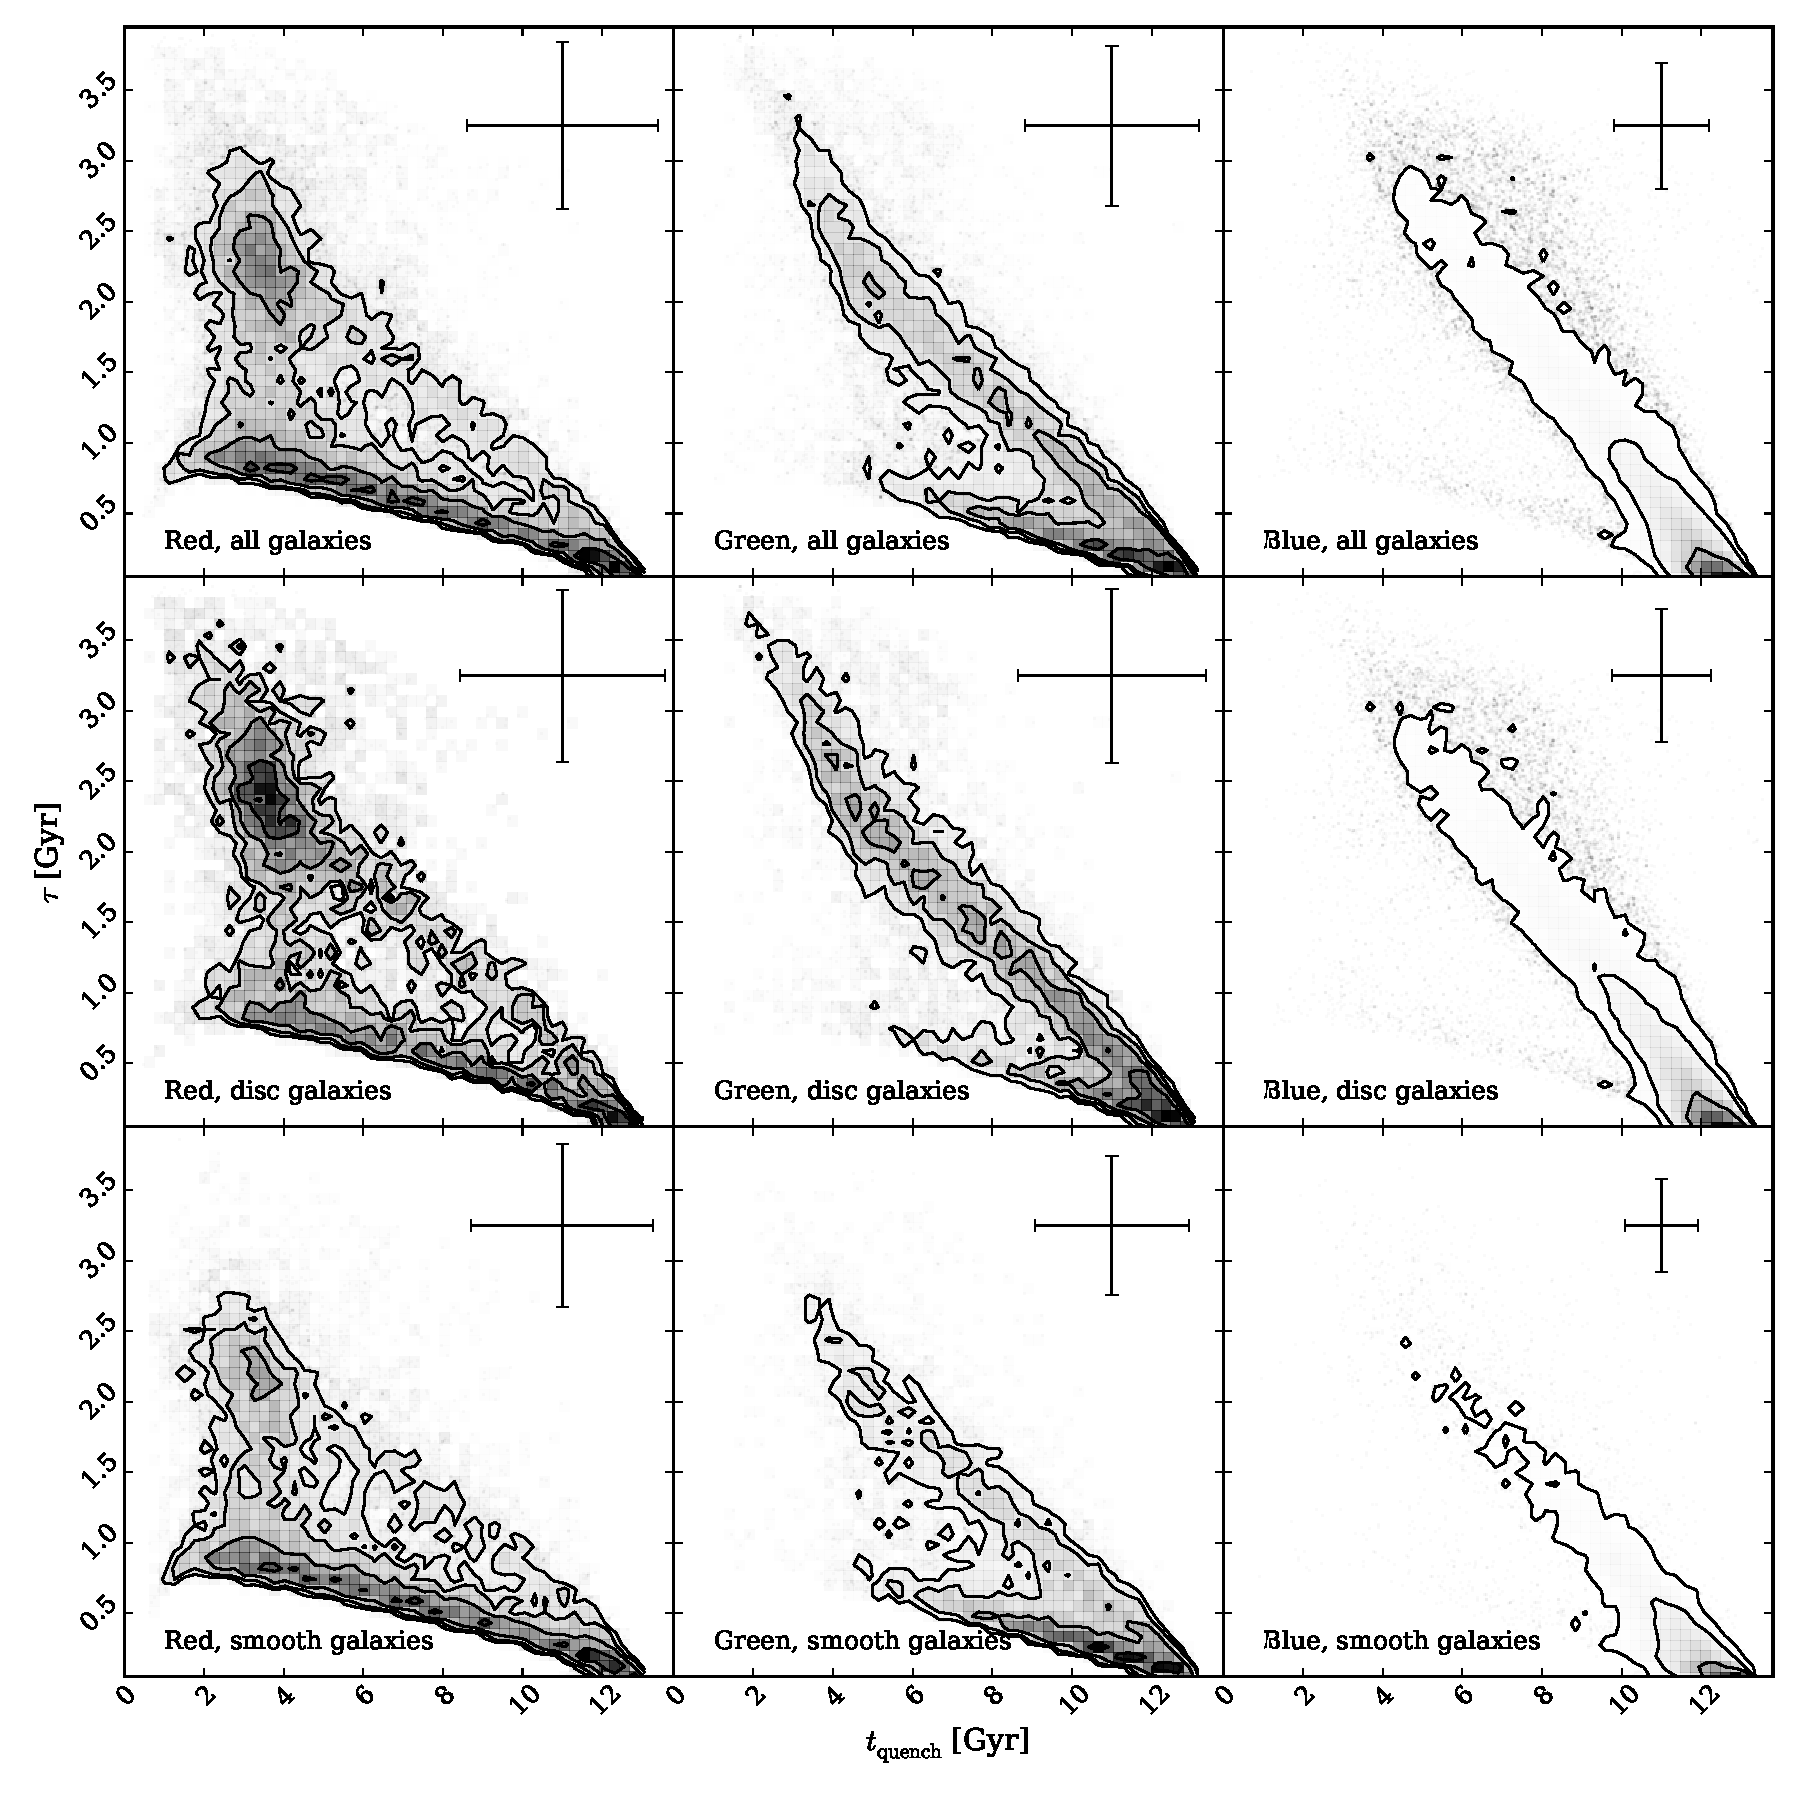
\includegraphics[width=0.95\textwidth]{morphology/contour_t_tau_mcmc_bestfit.pdf}
\caption[Best fit contours for red, green and blue clean galaxies]{Contours showing the positions in the $[t, \tau]$ parameter space of the median walker position (the 50th percentile; as shown by the intersection of the solid blue lines in Figure~\ref{one_example}) for each galaxy for all (top), disc ($p_d > 0.5$; middle), and smooth ($p_s > 0.5$; bottom) red sequence, green valley and blue cloud galaxies in the left, middle and bottom panels respectively. The error bars on each panel shows the average $68\%$ confidence on the median positions (calculated from the 16th and 84th percentile, as shown by the blue dashed lines in Figure~\ref{one_example}). These positions were calculated without discarding any walker positions due to low probability and without weighting by vote fractions, therefore this plot may be more intuitive than Figures~\ref{red_s},~\ref{green_v} \&~\ref{blue_c}. The differences between the smooth and disc populations and between the red, green and blue populations remain clearly apparent.}
\label{fig:bestfit}
\end{figure*}

Since the blue cloud is considered to be primarily made of star forming galaxies \starpy~ is expected to have some difficulty in determining the most likely quenching model to describe them, as confirmed by Figure~\ref{blue_c}. The attempt to characterise a star forming galaxy with a quenched SFH model leads \starpy~ to attribute the extremely blue colours of the majority of these galaxies with a constant SFR for as long as possible leading to fast quenching at the observed redshift (i.e. the colour has not had enough time to change from blue post quench; see the bottom panel of Figure~\ref{blue_c} in comparison with the bottom panel of Figure~\ref{pred}).

This is particularly apparent for the blue disc weighted population. Perhaps even galaxies which are currently quenching slowly across the blue cloud cannot be well fit by the quenching models implemented, as they still have high SFRs despite some quenching (by definition although a galaxy is undergoing quenching, star formation can still be occurring in a galaxy, just at a slower rate than at earlier times, described by $\tau$).


There is a very small preference for the blue smooth weighted population to undergo slow quenching which began prior to $z \sim 0.5 $. These populations have been blue for a considerable period of time, slowly using up their gas for star formation by the Kennicutt$-$Schmidt law \citep{Schmidt59, Kennicutt97}. However the major preference is for rapid quenching at recent times in the blue cloud; this therefore provides some support to the theories for blue ellipticals as either merger-driven ($\sim76\%$; like those identified as recently quenched ellipticals with properties consistent with a merger origin by \citealt{McIntosh14}) or gas inflow-driven reinvigorated star formation that is now slowly decreasing ($\sim24\%$; such as the population of blue spheroidal galaxies studied by \citealt{Kaviraj13}). However, remember that the quenching models used in this work do not provide an adequate fit to the blue cloud population.

The blue cloud is therefore primarily composed of both star forming galaxies of all morphologies and a smooth population which are undergoing a rapid quench, presumably after a previous event triggered star formation and turned them blue.


\section{Discussion}\label{morph:discussion}

In the previous section I presented the results of using \starpy ~to derive the most likely quenching histories for galaxies across the colour magnitude diagram and found differences between the SFHs of smooth- and disc-weighted populations of the red sequence, green valley and blue cloud. In this section I will speculate on the following question: what are the possible mechanisms driving these differences? 

\subsection{Rapid Quenching Mechanisms}\label{rapid}

Rapid quenching is much more prevalent in smooth galaxies than disc galaxies, and red galaxies are also much more likely to be characterised by a rapid quenching model than green valley galaxies (disregarding blue cloud galaxies due to their apparent poor fit by the quenching models, see Figure~\ref{blue_c}). In the green valley there is also a distinct lack of preference for rapid quenching timescales with $\tau < 0.5~\rm{Gyr}$; however the observability of a rapid quenching history declining with decreasing $\tau$ must be taken into account. Rapid mechanisms may be more common in the green valley than seen in Figure \ref{green_v}, however this observability should not depend on morphology so the conclusion that rapid quenching mechanisms are detected more for smooth rather than disc galaxies still holds. 

This suggests that rapid quenching mechanisms can cause a change in morphology from a disc- to a smooth dominated galaxy as it quickly traverses the colour-magnitude diagram to the red sequence. This is supported by the number of disc galaxies that would need to undergo a morphological change in order for the disc : smooth ratio of galaxies in the green valley to match that of the red galaxies in the \textsc{gz2-galex} sample (see Section~\ref{gv}). From this indirect evidence I suggest that this observed rapid quenching mechanism is caused by major mergers.

Inspection of the galaxies contributing to this area of population density reveals that this does not arise due to \emph{currently} merging pairs missed by GZ users which were not excluded from the \textsc{gz2-galex} sample (see Section \ref{class}), but by typical smooth galaxies with both red optical and NUV colours that \starpy~ attributes to rapid quenching at early times. Although a prescription for modelling a merger in the SFH is not included in this work the after effects can still be detected (see Section \ref{future} for future work planned with \starpy).

One simulation of interest by \citet{springel05b} showed that feedback from black hole activity is a necessary component of destructive major mergers to produce such rapid quenching timescales. Powerful quasar outflows can remove much of the gas from the inner regions of the galaxy, terminating star formation on extremely short timescales. \citet{Bell06}, using data from the COMBO-17 redshift survey ($0.4 < z < 0.8$), estimate a merger timescale from being classified as a close galaxy pair to recognisably disturbed as $\sim 0.4~\rm{Gyr}$. \citet{springel05b} consequently find using hydrodynamical simulations that after $\sim1~\rm{Gyr}$ the merger remnant has reddened to $u-r \sim 2.0$. This is in agreement with the simple exponential quenching models used here which show (Figure~\ref{sfr_mass_col}) that the models with a SFH with $\tau < 0.4~\rm{Gyr}$ have reached the red sequence, with $u-r ~\gtrsim 2.2$, within $\sim1~\rm{Gyr}$. This could explain the preference for red disc galaxies with rapid quenching timescales ($31.3\%$), as they may have undergone a major merger recently but are still undergoing a morphological change from disc, to disturbed, to an eventual smooth galaxy (see also \citealt{vdW09}) or have retained their disc structure in a merger in line with recent simulations from \citet{pontzen16}. This possible connection between AGN feedback and rapid quenching timescales is explored further in Chapter~\ref{agnfeedback}. 

This rapid quenching mechanism occurs much more rarely in green valley galaxies of both morphologies than for the subset of red sequence galaxies studied, however does not fully characterise all the galaxies in either the red sequence or green valley. Dry major mergers therefore do not fully account for the formation of any galaxy type at any redshift, supporting the observational conclusions made by \citet{Bell07,Bundy07, kaviraj14a} and simulations by \citet{Genel08}. 

\subsection{Intermediate Quenching Mechanisms}\label{int}

Intermediate quenching timescales are found to be equally prevalent across  all populations of both smooth and disc galaxies across cosmic time,  particularly in the green valley. Intermediate timescales are the prevalent mechanism for quenching smooth green valley galaxies, unlike the rapid quenching prevalent for red galaxies. This suggests that this intermediate quenching route must therefore be possible with routes that both preserve and transform morphology. It is this result of another route through the green valley that is in contradiction with the findings of S14. 

Once again considering the simulations of \citet{springel05b}, this time without any feedback from black holes, they suggest that if even a small fraction of gas is not consumed in the starburst following a merger (either because the mass ratio is not large enough or from the lack of strong black hole activity) the remnant can sustain star formation for periods of several Gyrs. The remnants from these simulations take $\sim5.5~\rm{Gyr}$ to reach red optical colours of $u-r \sim 2.1$. In Figure~\ref{sfr_mass_col} it can be seen that the models with intermediate quenching timescales of $1.0 \lesssim ~\tau~\rm{[Gyr]} ~\lesssim 2.0$ take approximately $2.5-5.5~\rm{Gyr}$ to reach these red colours. Similarly the recent simulations of \citet{pontzen16} show that without feedback the SFR of a disc galaxy can recover post merger and remain a star forming disc. 

I propose that the intermediate quenching timescales are caused by gas rich major mergers, major mergers without black hole feedback and from minor mergers, the latter of which being the dominant mechanism. This is supported by the findings of \citet{lotz08b} who find that the detectability timescales for equal mass gas rich mergers with large initial separations range from $\sim 1.1-1.9~\rm{Gyr}$, and of \citet{Lotz11}, who find in further simulations that as the baryonic gas fraction in a merger with mass ratios of 1:1-1:4 increases, so does the timescale of the merger from $\sim0.2~\rm{Gyr}$ (with little gas, as above for major mergers causing rapid quenching timescales) up to $\sim1.5~\rm{Gyr}$ (with large gas fractions). 

Here the very basic assumption is that the morphologically detectable timescale of a merger is roughly the same order as the quenching timescale. However, the existence of a substantial population of blue ellipticals \citep{Sch09} must be considered, which are thought to be post-merger systems with no detectable morphological signatures of a merger but with the merger-induced starburst still detectable in the photometry. This photometry is an indicator for the SFH and therefore should present with longer timescales for the photometric effects of a merger than found in the simulations by \citet{lotz08b} and \citet{Lotz11}. Observing this link between the timescale for the morphological observability of a merger and the timescales for the star formation induced by a merger is problematic, as evidenced by the lack of literature on the subject.

\citet{lotz08b} also show that the remnants of these simulated equal mass gas rich disc mergers (wet disc mergers) are observable for $\gtrsim1~\rm{Gyr}$ post merger and state that they appear ``disc-like and dusty" in the simulations, which is consistent with an ``early-type spiral morphology".  Such galaxies are often observed to have spiral features with a dominant bulge, suggesting that such galaxies may divide the votes of the GZ2 users, producing vote fractions of $p_s \sim p_d \sim 0.5$. This may be why the intermediate quenching timescales are equally dominant for both smooth and disc populations in Figures~\ref{red_s} and~\ref{green_v}. 

Other simulations (e.g. such as \citet{robertson06} and \citet{Barnes02}) support the conclusion that both gas rich major mergers and minor mergers can produce disc-like remnants. Observationally, \citet{Darg10a} showed an increase in the spiral to elliptical ratio for merging galaxies ($0.005 < z < 0.1$) by a factor of two compared to the general population. They attribute this to the much longer timescales during which mergers of spirals are observable compared to mergers with elliptical galaxies, confirming the hypothesis that the quenching timescales $\tau < 1.5 ~\rm{Gyr}$ preferred by disc galaxies may be undergoing mergers which will eventually lead to a morphological change. Similarly, \citet{Casteels13} observe that galaxies ($0.01 < z < 0.09$) which are interacting often retain their spiral structures and that a spiral galaxy which has been classified as having `loose winding arms' by the GZ2 users are often entering the early stages of mergers and interactions.

$40.6\%$ of the probability for smooth galaxies in the green valley arises due to intermediate quenching timescales (see Figure~\ref{green_v}); this is in agreement with work done by \citet{kaviraj14a, kaviraj14b} who by studying SDSS photometry ($z<0.07$) state that approximately half of the star formation in galaxies is driven by minor mergers at $0.5 < z < 0.7$ therefore exhausting available gas for star formation and consequently causing a gradual decline in the star formation rate. This supports earlier work by \cite{kaviraj11} who, using multi wavelength photometry of galaxies in COSMOS \citep{Scoville07}, found that $70\%$ of early-type galaxies appear morphologically disturbed, suggesting either a minor or major merger in their history. This is in agreement with the total percentage of the population density with $\tau < 2.0 ~\rm[Gyr]$; $73.9\%$ and $59.3\%$, for the smooth red and green galaxies in Figures~\ref{red_s} and~\ref{green_v} respectively. Note that the star formation model used here is a basic one and has no prescription for reignition of star formation post-quench which can also cause morphological disturbance of a galaxy, like those detected by \cite{kaviraj11} and seen in simulations by \cite{pontzen16}.

\citet{Darg10a} show in their Figure 6 that that beyond a merger ratio of $1:10$ (up to $\sim 1:100$), green is the dominant average galaxy colour of the visually identified merging pair in GZ. These mergers are also dominated by spiral-spiral mergers as opposed to elliptical-elliptical and elliptical-spiral. This supports the hypothesis that these intermediate timescales dominating in the green valley are caused in part by minor mergers. However this is contradictory to the findings of \citet{Mendez11} who find the merger fraction in the green valley is much lower than in the blue cloud, however they use an analytical light decomposition indicator to identify their mergers ($Gini/M_{20}$; see \citealt{lotz08b}), which tends to detect major mergers more easily than minor mergers. I have discussed the lower likelihood of a green valley galaxy to undergo a rapid quench, which I have hypothesised are attributed to major mergers (see Section \ref{rapid}), despite the caveat of the observability and believe that this may have been the phenomenon that \citet{Mendez11} detected.

The resultant intermediate quenching timescales occur initially due to one interaction mechanism, unlike the rapid quenching, which occurs due to a major merger combined with AGN feedback, and decreases the SFR over a short period of time. Therefore any external event which can cause either a burst of star formation (depleting the gas available) or directly strip a galaxy of its gas, for example galaxy harassment, interactions, ram pressure stripping, strangulation and interactions internal to clusters, would cause quenching on an intermediate timescale. Such mechanisms would be the dominant cause of quenching in dense environments; considering that the majority of galaxies reside in groups or clusters (\citealt{Coil08} find that green valley galaxies are just as clustered as red sequence galaxies). It is not surprising therefore that the majority of the \textsc{gz2-galex} galaxies are considered intermediate in morphology (see Table~\ref{table:subs}) and therefore are undergoing or have undergone such an interaction. This obvious dependancy of the quenching parameters with the galaxy environment will be investigated further in Chapter~\ref{chap:env}.


\subsection{Slow Quenching Timescales}\label{slow}
Although intermediate and rapid quenching timescales are the dominant mechanisms across the colour-magnitude diagram, together they cannot completely account for the quenching of disc galaxies. S14 concluded that slow quenching timescales were the most dominant mechanism for disc galaxies. However I show that: (i) intermediate quenching timescales are equally important in the green valley and (ii) rapid quenching timescales are equally important for the red galaxies with NUV emission. There is also a significantly lower preference for smooth galaxies to undergo such slow quenching timescales; suggesting that the evolution (or indeed creation) of typical smooth galaxies is dominated by processes external to the galaxy. This is excepting galaxies in the blue cloud where a small amount of slow evolution of blue ellipticals is occurring, presumably after a reinvigoration of star formation which is slowly depleting the gas available according to the Kennicutt$-$Schmidt law.

\citet{Bamford09} using GZ1 vote fractions of galaxies in the SDSS, found a significant fraction of high stellar mass red spiral galaxies in the field. As these galaxies are isolated from the effects of interactions from other galaxies, the slow quenching mechanisms present in their preferred star formation histories are most likely due to secular processes (i.e. mechanisms internal to the galaxy, in the absence of sudden accretion or merger events; \citealt{kormendy04, Sheth12}). Bar formation in a disc galaxy is such a mechanism, whereby gas is funnelled to the centre of the galaxy by the bar over long timescales where it is used for star formation \citep{masters12a, saintonge12, Cheung13}, consequently forming a `pseudo-bulge' \citep{Kormendy10, Simmons13}.

If these slow quenching timescales are due to secular evolution processes, this is to be expected since these processes do not change the disc dominated nature of a galaxy. 

\section{Conclusions}\label{morph:conc}

I have used morphological classifications from the Galaxy Zoo 2 project to determine the morphology-dependent star formation histories of galaxies via a Bayesian analysis of an exponentially declining star formation quenching model. The most likely parameters were determined for the quenching onset time, $t_q$ and quenching timescale $\tau$ in this model for galaxies across the blue cloud, green valley and red sequence to trace the morphological dependance of galactic evolution across the colour-magnitude diagram. The green valley is indeed found to be a transitional population for all morphological types (in agreement with \citet{schawinski14}), however this transition proceeds slowly for the majority of disc dominated galaxies and occurs rapidly for the majority of smooth dominated galaxies in the red sequence. However, in addition to \citet{schawinski14}, this Bayesian approach has revealed a more nuanced result, specifically that the prevailing mechanism across all morphologies and populations is quenching with intermediate timescales. The main findings are summarised as follows:
\begin{enumerate}[(i)]
\item The subset of red sequence galaxies with NUV emission studied in this investigation are found to have similar preferences for quenching timescales compared to green valley galaxies, but the quenching occurs at earlier quenching times (i.e. higher redshift) regardless of morphology (see Figures~\ref{red_s} and~\ref{green_v}). Therefore the quenching mechanisms currently occurring in the green valley were also active in creating the `blue end of of the red sequence' at earlier times; confirming that the green valley is indeed a transitional population, regardless of morphology.

\item The typical red galaxy with NUV emission studied, is elliptical in morphology and has undergone a rapid to intermediate quench at some point in cosmic time, resulting in a very low current SFR (see Section~\ref{rs}.

\item The green valley as it is currently observed is dominated by very slowly evolving disc dominated galaxies along with intermediate- and smooth dominated galaxies which pass across it with intermediate timescales within $\sim 1.0-1.5~\rm{Gyr}$ (see Section~\ref{gv}).

\item There are many different mechanisms responsible for quenching, all causing a galaxy to progress through the green valley, which are dependant on galaxy type, with the smooth and disc dominated galaxies each having different dominant star formation histories across the colour-magnitude diagram. These timescales can be roughly split into three main regimes; rapid ($\tau < 1.0~$Gyr), intermediate ($1.0 < \tau~$[Gyr]~$< 2.0$) and slow ($\tau > 2.0~$ Gyr) quenching.

\item Blue cloud galaxies are not well fit by a quenching model of star formation due to the continuous high star formation rates occurring (see Figure~\ref{blue_c}).

\item Rapid quenching timescales are detected with a lower probability for green valley galaxies than the red sequence galaxies studied. I speculate that this quenching mechanism is caused by major mergers with black hole feedback, which are able to expel the remaining gas not initially exhausted in the merger-induced starburst and which can cause a change in morphology from disc- to bulge-dominated. The colour-change timescales from previous simulations of such events agree with the derived timescales (see Section~\ref{rapid}). These rapid timescales are instrumental in forming red galaxies, however galaxies at the current epoch passing through the green valley do so at more intermediate timescales (see Figure~\ref{green_v}).

\item Intermediate quenching timescales ($1.0 < ~\tau~\rm{[Gyr]}~ < 2.0 $) are found with constant density across red and green galaxies for both smooth- and disc-weighted populations, the timescales for which agree with observed and simulated minor merger timescales (see Section~\ref{int}). I hypothesise that such timescales can be caused by a number of external processes, including gas rich major mergers, mergers without black hole feedback, galaxy harassment, interactions and ram pressure stripping. The timescales and observed morphologies from previous studies agree with the results, including that this is the dominant mechanisms for intermediate galaxies such as early-type spiral galaxies with spiral features but a dominant bulge, which split the GZ2 vote fractions (see Section~\ref{int}). 

\item Slow quenching timescales are the most dominant mechanism in the disc galaxy populations across the colour-magnitude diagram. Disc galaxies are often found in the field, therefore I hypothesise that such slow quenching timescales are caused by secular evolution and processes internal to the galaxy (see Section \ref{bc}). A small amount of slow quenching timescales is also detected for blue elliptical galaxies which is attributed to a reinvigoration of star formation, the peak of which has passed and has started to decline by slowly depleting the gas available (see Section~\ref{bc}). 
\end{enumerate}
